% ============================================================
%  Regulatory Watch — Technical Architecture Report
%  Generated: March 2026
% ============================================================
\documentclass[12pt,a4paper]{article}

% ── Packages ─────────────────────────────────────────────────────────────────
\usepackage[margin=2.5cm, headheight=15pt]{geometry}
\usepackage[T1]{fontenc}
\usepackage[utf8]{inputenc}
\usepackage{lmodern}
\usepackage{microtype}
\usepackage{parskip}
\usepackage{setspace}
\usepackage{titlesec}
\usepackage{titling}
\usepackage{fancyhdr}
\usepackage{xcolor}
\usepackage{hyperref}
\usepackage{listings}
\usepackage{booktabs}
\usepackage{longtable}
\usepackage{array}
\usepackage{multirow}
\usepackage{graphicx}
\usepackage{tikz}
\usetikzlibrary{shapes.geometric, arrows.meta, positioning, fit, backgrounds, calc, shapes.symbols}
\usepackage{enumitem}
\usepackage{tcolorbox}
\usepackage{amsmath}
\usepackage{tabularx}
\usepackage{float}

% ── Colour palette ───────────────────────────────────────────────────────────
\definecolor{primaryblue}{HTML}{1A3A5C}
\definecolor{accentblue}{HTML}{2E7BBF}
\definecolor{lightgray}{HTML}{F5F5F5}
\definecolor{darkgray}{HTML}{333333}
\definecolor{successgreen}{HTML}{2E8B57}
\definecolor{warnred}{HTML}{C0392B}
\definecolor{codebg}{HTML}{F8F8F8}
\definecolor{codefg}{HTML}{2C3E50}
\definecolor{commentgray}{HTML}{7F8C8D}
\definecolor{stringgreen}{HTML}{27AE60}
\definecolor{keywordpurple}{HTML}{8E44AD}

% ── Hyperref setup ────────────────────────────────────────────────────────────
\hypersetup{
    colorlinks=true,
    linkcolor=accentblue,
    urlcolor=accentblue,
    citecolor=accentblue,
    pdftitle={Regulatory Watch — Technical Architecture Report},
    pdfauthor={Engineering Team},
    pdfsubject={Architecture Documentation},
    pdfkeywords={regulatory, FastAPI, Celery, PostgreSQL, Kafka, ingestion},
}

% ── Listings (code blocks) ───────────────────────────────────────────────────
\lstdefinestyle{pythonstyle}{
    language=Python,
    backgroundcolor=\color{codebg},
    basicstyle=\ttfamily\small,
    keywordstyle=\color{keywordpurple}\bfseries,
    stringstyle=\color{stringgreen},
    commentstyle=\color{commentgray}\itshape,
    numberstyle=\tiny\color{commentgray},
    breakatwhitespace=false,
    breaklines=true,
    captionpos=b,
    keepspaces=true,
    numbers=left,
    numbersep=5pt,
    showspaces=false,
    showstringspaces=false,
    showtabs=false,
    tabsize=4,
    frame=single,
    rulecolor=\color{accentblue!30},
    xleftmargin=10pt,
    xrightmargin=5pt,
}

\lstdefinestyle{sqlstyle}{
    language=SQL,
    backgroundcolor=\color{codebg},
    basicstyle=\ttfamily\small,
    keywordstyle=\color{accentblue}\bfseries,
    stringstyle=\color{stringgreen},
    commentstyle=\color{commentgray}\itshape,
    breaklines=true,
    frame=single,
    rulecolor=\color{accentblue!30},
    xleftmargin=10pt,
}

\lstdefinestyle{shellstyle}{
    language=bash,
    backgroundcolor=\color{darkgray!90},
    basicstyle=\ttfamily\small\color{white},
    keywordstyle=\color{accentblue!80},
    stringstyle=\color{successgreen!80},
    commentstyle=\color{commentgray},
    breaklines=true,
    frame=single,
    rulecolor=\color{darkgray},
    xleftmargin=10pt,
}

\lstset{style=pythonstyle}

% ── Section formatting ────────────────────────────────────────────────────────
\titleformat{\section}
  {\Large\bfseries\color{primaryblue}}
  {\thesection}{1em}{}[\titlerule]

\titleformat{\subsection}
  {\large\bfseries\color{accentblue}}
  {\thesubsection}{1em}{}

\titleformat{\subsubsection}
  {\normalsize\bfseries\color{darkgray}}
  {\thesubsubsection}{1em}{}

% ── tcolorbox styles ──────────────────────────────────────────────────────────
\tcbuselibrary{skins, breakable}

\newtcolorbox{notebox}[1][Note]{
  colback=accentblue!8,
  colframe=accentblue,
  fonttitle=\bfseries,
  title=#1,
  breakable,
}

\newtcolorbox{warnbox}[1][Warning]{
  colback=warnred!8,
  colframe=warnred,
  fonttitle=\bfseries,
  title=#1,
  breakable,
}

\newtcolorbox{successbox}[1][Status]{
  colback=successgreen!8,
  colframe=successgreen,
  fonttitle=\bfseries,
  title=#1,
  breakable,
}

% ── Header / Footer ───────────────────────────────────────────────────────────
\pagestyle{fancy}
\fancyhf{}
\fancyhead[L]{\small\color{primaryblue}\textbf{Regulatory Watch}}
\fancyhead[R]{\small\color{darkgray}Technical Architecture Report}
\fancyfoot[C]{\small\color{darkgray}\thepage}
\renewcommand{\headrulewidth}{0.4pt}
\renewcommand{\footrulewidth}{0.2pt}

% ── Title page ────────────────────────────────────────────────────────────────
\title{%
  {\color{primaryblue}\Huge\bfseries Regulatory Watch}\\[0.5em]
  {\color{accentblue}\Large Technical Architecture \& State Report}\\[0.3em]
  {\color{darkgray}\normalsize Version 0.1.0 --- March 2026}
}
\author{Engineering Team}
\date{\today}

% ─────────────────────────────────────────────────────────────────────────────
\begin{document}

\maketitle
\thispagestyle{empty}

\vspace{1cm}

\begin{abstract}
\noindent
This document provides a comprehensive technical description of the \textbf{Regulatory Watch} platform, an AI-assisted regulatory monitoring system. It covers the application purpose and business rationale, the full distributed architecture, all five data ingestion connectors (Web, RSS, PDF, XML, and Email), the complete database schema, URL normalisation and spider-trap detection mechanisms, content deduplication strategy, S3 artifact storage design, current data collection status (188 documents collected as of March 2026), monitored regulatory sources, and an honest assessment of implemented versus planned capabilities. The document is intended for developers, architects, and technical stakeholders who need a single authoritative reference for the system.
\end{abstract}

\vspace{1cm}
\tableofcontents
\clearpage

% ═════════════════════════════════════════════════════════════════════════════
\section{Introduction and Purpose}
% ═════════════════════════════════════════════════════════════════════════════

\subsection{What is Regulatory Watch?}

Regulatory Watch is a continuous regulatory intelligence platform designed to monitor, ingest, deduplicate, and eventually analyse regulatory publications from financial and legislative authorities around the world. The system automatically watches official government and regulatory body websites, RSS feeds, structured XML publications, PDF documents, and email alerts, collecting regulatory text as soon as it is published and making it available for downstream processing.

The platform targets compliance teams, legal analysts, and financial institutions that need timely, structured access to regulatory changes without manually visiting dozens of official websites every day.

\subsection{Business Motivation}

The volume of regulatory output from bodies such as the UK's Financial Conduct Authority (FCA), the European Union through EUR-Lex, and the United States Federal Register has grown substantially over the last decade. Missing a regulatory change can result in compliance failures, fines, and reputational damage. Manual monitoring is unreliable and expensive. Regulatory Watch addresses this by:

\begin{itemize}[noitemsep]
  \item Polling official feeds and websites on configurable schedules.
  \item Normalising and deduplicating content so analysts see each unique regulatory item exactly once.
  \item Storing raw artifacts for audit purposes.
  \item Providing a structured database that downstream AI analysis and alerting services can consume.
\end{itemize}

\subsection{Current Development Stage}

As of March 2026, the platform is in an active early-development phase. The data ingestion layer, deduplication engine, database schema, and background task infrastructure are fully operational. The platform has already collected \textbf{188 regulatory documents} from three jurisdictions. Higher-level capabilities—full-text search, AI-powered summarisation, change-diffing, and user-facing alerting—are planned for future sprints and are explicitly documented in Section~\ref{sec:roadmap}.

% ═════════════════════════════════════════════════════════════════════════════
\section{Technology Stack}
% ═════════════════════════════════════════════════════════════════════════════

Table~\ref{tab:techstack} lists every technology used in the platform.

\begin{longtable}{@{}p{4cm} p{3cm} p{7.5cm}@{}}
\caption{Technology Stack}\label{tab:techstack}\\
\toprule
\textbf{Component} & \textbf{Version} & \textbf{Role} \\
\midrule
\endfirsthead
\toprule
\textbf{Component} & \textbf{Version} & \textbf{Role} \\
\midrule
\endhead
\midrule
\multicolumn{3}{r}{\small\textit{Continued on next page\ldots}}
\endfoot
\bottomrule
\endlastfoot
Python                & 3.11             & Primary runtime language \\
FastAPI               & 0.115.6          & REST API framework; auto-generates OpenAPI docs \\
Uvicorn               & 0.34.0           & ASGI server; serves the FastAPI application \\
SQLModel              & 0.0.22           & ORM bridging SQLAlchemy + Pydantic; defines table models \\
PostgreSQL            & 16 (Alpine)      & Primary relational store for documents and metadata \\
psycopg2-binary       & 2.9.10           & PostgreSQL driver for SQLAlchemy \\
Alembic               & 1.14.1           & Database schema migration manager \\
Celery                & 5.4.0            & Distributed task queue; runs ingestion jobs \\
Redis                 & 7 (Alpine)       & Celery broker and result backend \\
Celery Beat           & (built-in)       & Periodic task scheduler embedded in the worker \\
Flower                & 2.0.1            & Real-time Celery monitoring dashboard \\
Apache Kafka          & 7.6.0 (Confluent)& Event streaming bus (future AI pipeline integration) \\
Zookeeper             & 7.6.0 (Confluent)& Kafka coordination service \\
Crawl4AI              & $\geq$0.4.0     & Playwright-based async web crawler; handles JS rendering \\
Playwright / Chromium & (via Crawl4AI)   & Headless browser for JS-rendered regulatory pages \\
pdfplumber            & $\geq$0.11.0    & Layout-aware PDF text and table extraction \\
feedparser            & $\geq$6.0.11    & RSS 0.9--2.0, Atom, and RDF feed parsing \\
lxml                  & (transitive)     & USLM and Akoma Ntoso XML parsing via XPath \\
httpx                 & 0.28.1           & Async HTTP client for robots.txt, PDF and XML fetching \\
langdetect            & $\geq$1.0.9     & ISO 639-1 language detection (local, no API key) \\
boto3                 & $\geq$1.34.0    & AWS SDK; S3 artifact storage (optional) \\
kafka-python-ng       & 2.2.3            & Kafka producer/consumer Python client \\
pydantic-settings     & 2.7.1            & Typed environment-variable configuration \\
python-json-logger    & 3.2.1            & Structured JSON log output \\
Docker / Compose      & (latest)         & Container orchestration for all services \\
OpenRouter / Qwen     & API              & LLM fallback for sparse web page extraction \\
\end{longtable}

% ═════════════════════════════════════════════════════════════════════════════
\section{System Architecture}
% ═════════════════════════════════════════════════════════════════════════════

\subsection{Architectural Overview}

Regulatory Watch follows a \textbf{microservice-inspired, event-driven architecture} deployed entirely in Docker containers via Docker Compose. The system decomposes into five logical tiers:

\begin{enumerate}[noitemsep]
  \item \textbf{API Tier} — FastAPI application serving REST endpoints.
  \item \textbf{Worker Tier} — Celery worker executing ingestion tasks; Celery Beat schedules periodic polls.
  \item \textbf{Data Tier} — PostgreSQL (structured storage) and Redis (broker/cache).
  \item \textbf{Streaming Tier} — Apache Kafka with Zookeeper (event bus, reserved for AI pipeline).
  \item \textbf{Artifact Tier} — AWS S3 (raw HTML and extracted text storage).
\end{enumerate}

\subsection{Service Map}

Figure~\ref{fig:architecture} shows the Docker Compose service topology.

\begin{figure}[H]
\centering
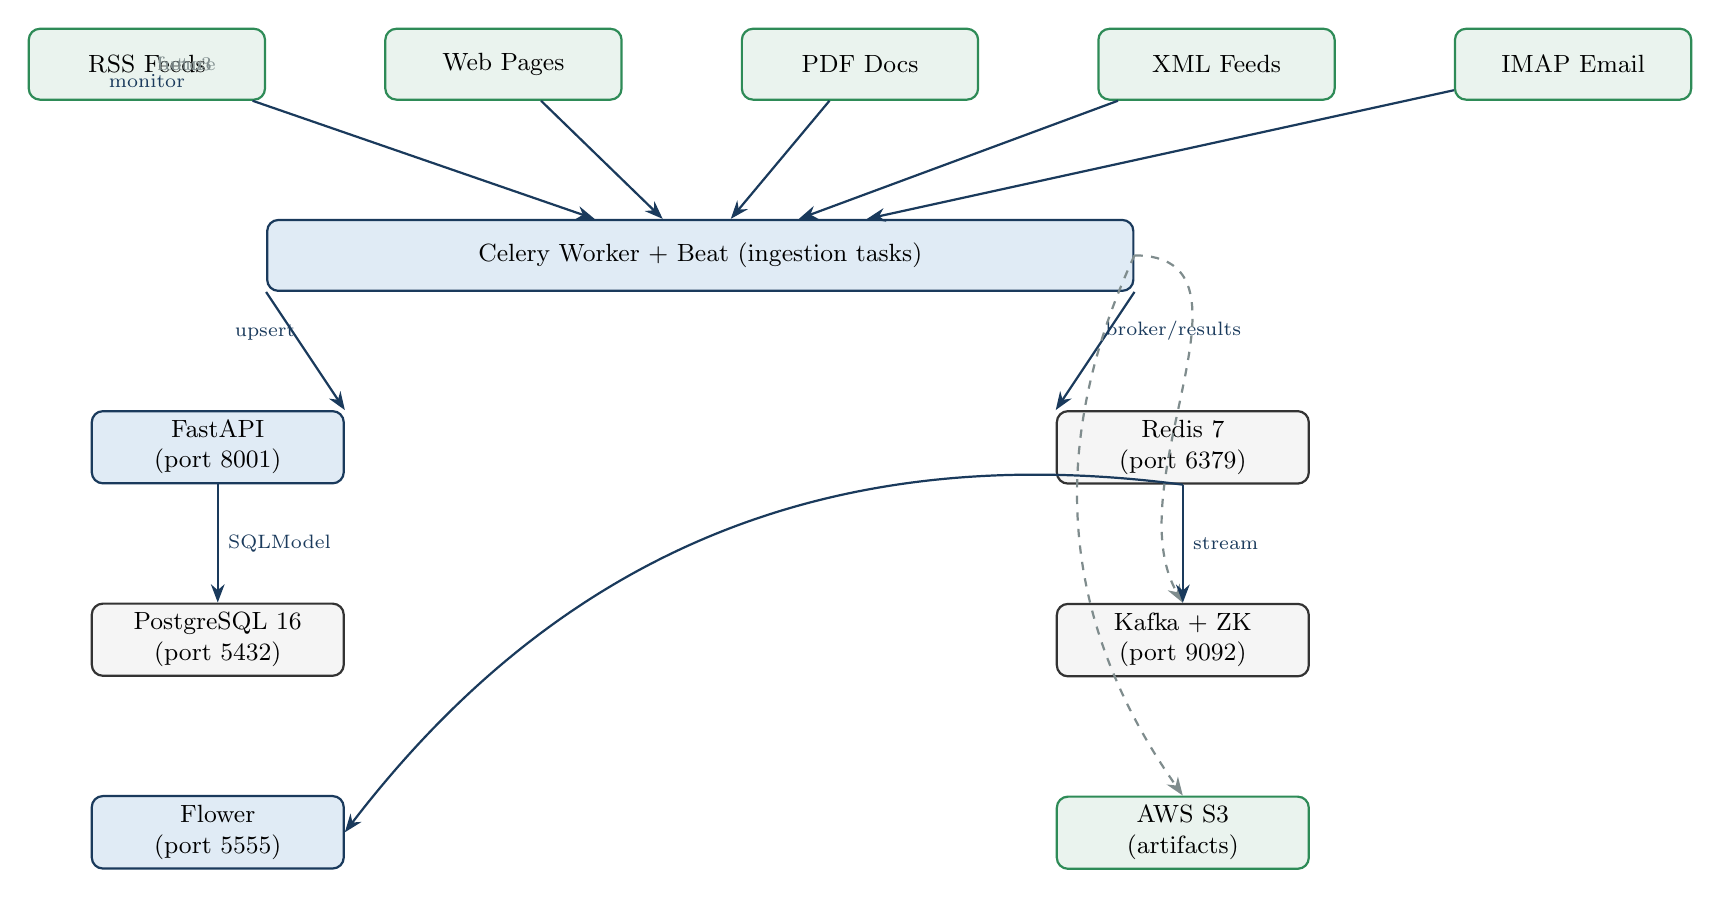
\begin{tikzpicture}[
  node distance=1.4cm and 2cm,
  every node/.style={font=\small},
  service/.style={
    rectangle, rounded corners=4pt,
    minimum width=3cm, minimum height=0.9cm,
    align=center, draw=primaryblue, thick,
    fill=accentblue!15,
  },
  external/.style={
    rectangle, rounded corners=4pt,
    minimum width=3cm, minimum height=0.9cm,
    align=center, draw=successgreen, thick,
    fill=successgreen!10,
  },
  infra/.style={
    rectangle, rounded corners=4pt,
    minimum width=3cm, minimum height=0.9cm,
    align=center, draw=darkgray, thick,
    fill=lightgray,
  },
  arrow/.style={-Stealth, thick, color=primaryblue},
  dasharrow/.style={-Stealth, dashed, thick, color=commentgray},
]

% Row 1 — external sources
\node[external] (rss)     {RSS Feeds};
\node[external, right=1.5cm of rss]  (web)     {Web Pages};
\node[external, right=1.5cm of web]  (pdf)     {PDF Docs};
\node[external, right=1.5cm of pdf]  (xml)     {XML Feeds};
\node[external, right=1.5cm of xml]  (email)   {IMAP Email};

% Row 2 — worker
\node[service, below=1.5cm of web,
      minimum width=11cm,
      xshift=2.5cm]
      (worker)  {Celery Worker + Beat (ingestion tasks)};

% Row 3 — API and broker side-by-side
\node[service, below left=1.5cm and -1cm of worker,
      minimum width=3.2cm]     (api)     {FastAPI\\(port 8001)};
\node[infra, below right=1.5cm and -1cm of worker,
      minimum width=3.2cm]     (redis)   {Redis 7\\(port 6379)};

% Row 4 — databases / stream
\node[infra, below=1.5cm of api,
      minimum width=3.2cm]     (pg)      {PostgreSQL 16\\(port 5432)};
\node[infra, below=1.5cm of redis,
      minimum width=3.2cm]     (kafka)   {Kafka + ZK\\(port 9092)};

% Row 5 — monitoring + S3
\node[service, below=1.5cm of pg,
      minimum width=3.2cm]     (flower)  {Flower\\(port 5555)};
\node[external, below=1.5cm of kafka,
      minimum width=3.2cm]     (s3)      {AWS S3\\(artifacts)};

% Arrows — external to worker
\draw[arrow] (rss)   -- (worker);
\draw[arrow] (web)   -- (worker);
\draw[arrow] (pdf)   -- (worker);
\draw[arrow] (xml)   -- (worker);
\draw[arrow] (email) -- (worker);

% Worker <-> Redis (broker)
\draw[arrow] (worker.south east) -- (redis.north west)
  node[midway, above right, font=\scriptsize]{broker/results};

% Worker -> PostgreSQL
\draw[arrow] (worker.south west) -- (api.north east)
  node[midway, above left, font=\scriptsize]{upsert};
\draw[arrow] (api) -- (pg)
  node[midway, right, font=\scriptsize]{SQLModel};

% Worker -> S3
\draw[dasharrow] (worker.east) to[bend right=30] (s3.north)
  node[midway, right, font=\scriptsize]{boto3};

% Worker -> Kafka (future)
\draw[dasharrow] (worker.east) to[out=0,in=120] (kafka.north)
  node[pos=0.5, right, font=\scriptsize]{future};

% Redis -> Flower
\draw[arrow] (redis) -- (kafka)
  node[midway, right, font=\scriptsize]{stream};
\draw[arrow] (redis.south) to[bend right=30] (flower.east)
  node[midway, below, font=\scriptsize]{monitor};

\end{tikzpicture}
\caption{Regulatory Watch service topology}\label{fig:architecture}
\end{figure}

\subsection{Docker Compose Services}

The \texttt{docker-compose.yml} defines seven containers shown in Table~\ref{tab:services}.

\begin{table}[H]
\centering
\caption{Docker Compose Services}\label{tab:services}
\begin{tabularx}{\textwidth}{@{}l l l X@{}}
\toprule
\textbf{Service} & \textbf{Image / Build} & \textbf{Host Port} & \textbf{Description} \\
\midrule
\texttt{db}         & postgres:16-alpine   & 5432  & PostgreSQL primary data store \\
\texttt{redis}      & redis:7-alpine       & 6379  & Celery broker and result backend \\
\texttt{zookeeper}  & cp-zookeeper:7.6.0   & 2181  & Kafka coordination \\
\texttt{kafka}      & cp-kafka:7.6.0       & 9092  & Event streaming (reserved) \\
\texttt{api}        & ./Dockerfile         & 8001  & FastAPI application (port 8000 internal) \\
\texttt{worker}     & ./Dockerfile         & ---   & Celery worker + Beat scheduler \\
\texttt{flower}     & ./Dockerfile         & 5555  & Celery task monitoring UI \\
\bottomrule
\end{tabularx}
\end{table}

\subsubsection{Health Checks}

PostgreSQL and Redis both declare health-check commands in Compose. The \texttt{api} and \texttt{worker} services declare \texttt{depends\_on} conditions that wait for healthy status before starting, preventing premature boot failures.

\begin{lstlisting}[style=shellstyle, caption={PostgreSQL health check}]
pg_isready -U regwatch
\end{lstlisting}

\subsubsection{Celery Worker and Beat Co-location}

The Celery worker and Beat scheduler run as a \textbf{single process} using the \texttt{--beat} flag:

\begin{lstlisting}[style=shellstyle, caption={Worker start command}]
celery -A app.celery_app:celery worker --loglevel=info --beat
\end{lstlisting}

This simplifies deployment for the current single-replica setup. In production, Beat would be separated into its own container to avoid Beat running on multiple replicas.

\subsection{FastAPI Application Structure}

The \texttt{api} service runs under Uvicorn with hot-reload enabled (\texttt{--reload}) and exposes the following routers:

\begin{table}[H]
\centering
\caption{FastAPI Routers and Endpoints}\label{tab:routers}
\begin{tabularx}{\textwidth}{@{}l l X@{}}
\toprule
\textbf{Router} & \textbf{Prefix} & \textbf{Endpoints} \\
\midrule
health.py   & \texttt{/health}  & \texttt{GET /health}, \texttt{GET /health/db}, \texttt{GET /health/redis} \\
domains.py  & \texttt{/domains} & \texttt{POST}, \texttt{GET} (list), \texttt{GET /\{id\}}, \texttt{PATCH /\{id\}}, \texttt{DELETE /\{id\}} \\
(root)      & \texttt{/}        & \texttt{GET /} — returns app name, version, and docs URL \\
\bottomrule
\end{tabularx}
\end{table}

Interactive API documentation is automatically available at \texttt{http://localhost:8001/docs} (Swagger UI) and \texttt{http://localhost:8001/redoc} (ReDoc).

\subsection{Kafka Integration (Reserved)}

Apache Kafka (Confluent Platform 7.6.0) with Zookeeper is fully provisioned and running in the Docker Compose stack. Auto-topic creation is enabled. The Kafka broker is available at \texttt{kafka:29092} (internal) and \texttt{localhost:9092} (host). At present, no Celery task publishes to Kafka. The infrastructure is reserved for a planned AI analysis pipeline that will consume raw documents from the \texttt{raw\_documents} topic and publish structured analysis results.

% ═════════════════════════════════════════════════════════════════════════════
\section{Database Schema}
% ═════════════════════════════════════════════════════════════════════════════

\subsection{Migration History}

The schema is managed by Alembic with the following migration chain:

\begin{itemize}[noitemsep]
  \item \textbf{Migration 001} (\texttt{2026-03-24}): Initial schema — \texttt{domains}, \texttt{urls}, \texttt{fetch\_runs}, \texttt{fetch\_attempts}.
  \item \textbf{Migration 002} (\texttt{2026-03-24}): Add \texttt{raw\_documents} table for the ingestion layer.
\end{itemize}

\subsection{Tables Overview}

The database contains five tables. Table~\ref{tab:tables} summarises their purpose and approximate row counts as of March 2026.

\begin{table}[H]
\centering
\caption{Database Tables}\label{tab:tables}
\begin{tabularx}{\textwidth}{@{}l X l@{}}
\toprule
\textbf{Table} & \textbf{Purpose} & \textbf{Rows (approx.)} \\
\midrule
\texttt{domains}         & Regulatory domains to monitor (seed URLs, rate limits) & small \\
\texttt{urls}            & Individual pages within a domain; BFS frontier management & small \\
\texttt{fetch\_runs}     & Batch crawl execution records & small \\
\texttt{fetch\_attempts} & Per-URL fetch records within a run; links to S3 artifacts & small \\
\texttt{raw\_documents}  & Ingested regulatory text from all connectors & \textbf{188} \\
\bottomrule
\end{tabularx}
\end{table}

\subsection{The \texttt{raw\_documents} Table}

This is the primary output table of the ingestion layer. Every unique piece of regulatory content — regardless of source type — lands here.

\begin{table}[H]
\centering
\caption{\texttt{raw\_documents} Table Schema}\label{tab:rawdoc}
\begin{tabularx}{\textwidth}{@{}l l l X@{}}
\toprule
\textbf{Column} & \textbf{Type} & \textbf{Nullable} & \textbf{Description} \\
\midrule
\texttt{id}            & UUID            & NOT NULL & Primary key (UUID v4, auto-generated) \\
\texttt{source\_url}   & TEXT            & NOT NULL & Canonical URL or identifier of the source \\
\texttt{source\_type}  & VARCHAR(20)     & NOT NULL & One of: \texttt{web}, \texttt{pdf}, \texttt{rss}, \texttt{xml}, \texttt{email} \\
\texttt{raw\_text}     & TEXT            & NULL     & Full extracted body text \\
\texttt{title}         & TEXT            & NULL     & Document title or section heading \\
\texttt{language}      & VARCHAR(10)     & NULL     & ISO 639-1 language code (e.g.\ \texttt{en}, \texttt{fr}) \\
\texttt{content\_hash} & VARCHAR(64)     & NOT NULL & SHA-256 hex of \texttt{raw\_text}; UNIQUE constraint \\
\texttt{fetched\_at}   & TIMESTAMPTZ     & NOT NULL & When this document was first collected \\
\texttt{last\_seen\_at}& TIMESTAMPTZ     & NOT NULL & When this content hash was last confirmed present \\
\bottomrule
\end{tabularx}
\end{table}

\subsubsection{Constraints and Indexes}

\begin{lstlisting}[style=sqlstyle, caption={raw\_documents DDL (from Alembic migration 002)}]
CREATE TABLE raw_documents (
    id            UUID         PRIMARY KEY,
    source_url    TEXT         NOT NULL,
    source_type   VARCHAR(20)  NOT NULL,
    raw_text      TEXT,
    title         TEXT,
    language      VARCHAR(10),
    content_hash  VARCHAR(64)  NOT NULL,
    fetched_at    TIMESTAMPTZ  NOT NULL,
    last_seen_at  TIMESTAMPTZ  NOT NULL,

    CONSTRAINT uq_raw_document_content_hash
        UNIQUE (content_hash),
    CONSTRAINT ck_raw_document_source_type
        CHECK (source_type IN ('web','pdf','rss','xml','email'))
);

CREATE INDEX ix_raw_documents_source_type  ON raw_documents (source_type);
CREATE INDEX ix_raw_documents_fetched_at   ON raw_documents (fetched_at);
CREATE INDEX ix_raw_documents_content_hash ON raw_documents (content_hash);
\end{lstlisting}

The \texttt{UNIQUE} constraint on \texttt{content\_hash} is the enforcement anchor of the deduplication strategy (see Section~\ref{sec:dedup}). The three secondary indexes support efficient queries by source type, time range, and hash lookup.

\subsection{The \texttt{domains} Table}

Stores the set of domains under active monitoring. Each row carries a JSON array of seed URLs that the web crawler uses as starting points, plus a rate limit expressed in requests per second.

Key columns: \texttt{id} (UUID PK), \texttt{domain} (unique string, e.g.\ \texttt{fca.org.uk}), \texttt{seed\_urls} (JSON array), \texttt{status} (\texttt{active} / \texttt{paused} / \texttt{archived}), \texttt{rate\_limit\_rps} (float).

\subsection{The \texttt{urls} Table}

Implements a per-domain URL frontier for the web crawler. Each discovered URL progresses through a state machine: \texttt{discovered} $\to$ \texttt{queued} $\to$ \texttt{fetched} (or \texttt{failed} / \texttt{ignored} / \texttt{blocked}). Key scoring columns include \texttt{priority}, \texttt{relevance\_score}, \texttt{hub\_score}, and \texttt{trap\_score}. Scheduling is managed via \texttt{next\_fetch\_at} and \texttt{fetch\_interval\_hours} (default: 168 hours = weekly).

\subsection{The \texttt{fetch\_runs} and \texttt{fetch\_attempts} Tables}

\texttt{fetch\_runs} records each batch crawl execution per domain (start time, finish time, counts of planned/fetched/changed/alerted URLs, and status). \texttt{fetch\_attempts} records the result of fetching a single URL within a run: HTTP status code, content hash, diff status, and S3 URIs for the stored raw HTML and extracted text.

% ═════════════════════════════════════════════════════════════════════════════
\section{Data Ingestion Layer}
% ═════════════════════════════════════════════════════════════════════════════

\subsection{Design Principles}

The ingestion layer is built around a single abstract base class, \texttt{IngestorBase} (task T2.1), located in \linebreak\texttt{app/ingestion/base.py}. All five connectors inherit from it and implement one async method:

\begin{lstlisting}[caption={IngestorBase interface}]
class IngestorBase(ABC):
    @abstractmethod
    async def fetch(self) -> List[RawDocument]:
        """
        Pull content from the source.
        content_hash (SHA-256 of raw_text) must be populated
        before returning so the storage layer can deduplicate.
        """
        ...
\end{lstlisting}

The caller (a Celery task) invokes \texttt{connector.fetch()}, receives a list of \texttt{RawDocument} instances, and hands them to \texttt{upsert\_documents()} in \texttt{app/ingestion/storage.py}. The connector is entirely unaware of persistence details; it only extracts and normalises.

\subsection{Connector 1 — WebConnector (T2.2)}

\subsubsection{Purpose}

The WebConnector performs a \textbf{breadth-first crawl} of a regulatory website, handling JavaScript-rendered pages, respecting robots.txt, enforcing rate limits, and applying spider-trap protection. It is the most complex of the five connectors.

\subsubsection{Implementation}

\begin{itemize}[noitemsep]
  \item \textbf{Library:} Crawl4AI with Playwright Chromium backend.
  \item \textbf{Content extraction:} Crawl4AI's Readability-style markdown processor strips navigation, footers, and ads. If the result is fewer than 200 characters, the system falls back to an LLM (Qwen via OpenRouter) that extracts the main regulatory body text.
  \item \textbf{Link discovery:} Internal links from the crawled page are normalised and enqueued for BFS traversal up to \texttt{max\_depth} (default: 3).
  \item \textbf{Compliance:} robots.txt is fetched and cached once per host per crawl run. URLs blocked by robots.txt are skipped. A configurable \texttt{rate\_limit\_rps} parameter inserts \texttt{asyncio.sleep} between requests.
\end{itemize}

\subsubsection{Configuration Parameters}

\begin{table}[H]
\centering
\caption{WebConnector Parameters}\label{tab:webparams}
\begin{tabularx}{\textwidth}{@{}l l l X@{}}
\toprule
\textbf{Parameter} & \textbf{Type} & \textbf{Default} & \textbf{Description} \\
\midrule
\texttt{seed\_urls}       & list[str] & ---  & Starting URLs for BFS \\
\texttt{allowed\_domain}  & str       & ---  & Domain boundary (subdomains allowed) \\
\texttt{max\_pages}       & int       & 50   & Hard cap on pages per run \\
\texttt{max\_depth}       & int       & 3    & BFS depth limit from seeds \\
\texttt{rate\_limit\_rps} & float     & 1.0  & Maximum requests per second \\
\bottomrule
\end{tabularx}
\end{table}

\subsubsection{Scheduled Runs (Celery Beat)}

\begin{table}[H]
\centering
\caption{Scheduled Web Crawl Jobs}\label{tab:webschedule}
\begin{tabularx}{\textwidth}{@{}l l X@{}}
\toprule
\textbf{Domain} & \textbf{Schedule} & \textbf{Seed URL} \\
\midrule
EUR-Lex         & Every 6 hours & \texttt{https://eur-lex.europa.eu/latest-laws/} \\
FCA             & Every 6 hours & \texttt{https://www.fca.org.uk/news} \\
Federal Register& Every 6 hours & \texttt{https://www.federalregister.gov/documents/current} \\
\bottomrule
\end{tabularx}
\end{table}

\subsection{Connector 2 — RSSConnector (T2.4)}

\subsubsection{Purpose}

The RSSConnector polls RSS 0.9--2.0, Atom, and RDF feeds and turns each entry into a \texttt{RawDocument} with \texttt{source\_type="rss"}.

\subsubsection{Implementation}

\begin{itemize}[noitemsep]
  \item \textbf{Library:} \texttt{feedparser} (supports all major feed formats, handles malformed feeds gracefully via \texttt{bozo} flag).
  \item \textbf{Since feedparser is synchronous}, it runs in a thread pool via \texttt{asyncio.run\_in\_executor}.
  \item \textbf{Text assembly:} Title, publication date (ISO 8601), summary, and link are joined into a single \texttt{raw\_text} string. This provides consistent, searchable content per entry.
  \item \textbf{Date parsing:} Attempts \texttt{published\_parsed} and \texttt{updated\_parsed} (time structs), then falls back to raw RFC 2822 string parsing.
  \item \textbf{Language detection:} \texttt{langdetect} analyses up to the first 2000 characters.
  \item \textbf{In-run deduplication:} A \texttt{seen\_hashes} set prevents duplicate entries within a single poll cycle before the data even reaches the database.
  \item \textbf{Max entries:} Capped at 100 entries per poll to avoid overwhelming the database on first run of a high-volume feed.
\end{itemize}

\subsubsection{Scheduled Runs}

\begin{table}[H]
\centering
\caption{Scheduled RSS Jobs}\label{tab:rssschedule}
\begin{tabularx}{\textwidth}{@{}l l l@{}}
\toprule
\textbf{Feed Name} & \textbf{Schedule} & \textbf{Feed URL} \\
\midrule
Federal Register & Every 30 minutes & \texttt{https://www.govinfo.gov/rss/fr.xml} \\
FCA News         & Every 30 minutes & \texttt{https://www.fca.org.uk/news/rss.xml} \\
\bottomrule
\end{tabularx}
\end{table}

\subsection{Connector 3 — PDFConnector (T2.3)}

\subsubsection{Purpose}

The PDFConnector fetches a PDF document from an HTTP(S) URL or local file path and extracts text and tables, producing \textbf{one \texttt{RawDocument} per page}.

\subsubsection{Implementation}

\begin{itemize}[noitemsep]
  \item \textbf{Primary extractor:} IBM Docling, when installed. Docling provides layout-aware extraction with superior table structure understanding. The entire document is returned as a single markdown-formatted chunk.
  \item \textbf{Fallback extractor:} \texttt{pdfplumber}, which processes the PDF page by page. Non-table text is extracted with \texttt{page.extract\_text()}, and tables are extracted with \texttt{page.extract\_tables()} then rendered as comma-separated rows — preventing cells from being merged into a single unreadable string.
  \item \textbf{Page filtering:} Pages with fewer than 50 characters of extracted text are discarded.
  \item \textbf{Download:} httpx with a 60-second timeout, following redirects, using the \texttt{RegulatoryWatch/1.0} user agent.
\end{itemize}

\subsubsection{Table Rendering}

\begin{lstlisting}[caption={Table-to-text rendering (pdfplumber)}]
def _table_to_text(table: list) -> str:
    lines = []
    for row in table:
        if row:
            cells = [str(c).strip() for c in row
                     if c is not None and str(c).strip()]
            if cells:
                lines.append(", ".join(cells))
    return "\n".join(lines)
\end{lstlisting}

Each table in the extracted text is surrounded by \texttt{--- TABLE ---} / \texttt{--- END TABLE ---} markers, making it easy for downstream parsers to detect tabular regions.

\subsubsection{Schedule}

PDF ingestion is triggered on-demand via the \texttt{pdf\_ingest\_task} Celery task. No periodic Beat schedule is currently defined for PDF sources; PDFs are submitted manually or triggered via API calls.

\subsection{Connector 4 — XMLConnector (T2.5)}

\subsubsection{Purpose}

The XMLConnector parses structured regulatory XML and produces one \texttt{RawDocument} per logical section or article.

\subsubsection{Supported XML Standards}

\begin{table}[H]
\centering
\caption{XML Standards Supported}\label{tab:xmlstds}
\begin{tabularx}{\textwidth}{@{}l l X@{}}
\toprule
\textbf{Standard} & \textbf{Namespace} & \textbf{Used by} \\
\midrule
USLM & \texttt{http://schemas.gpo.gov/xml/uslm} & US Code, Federal Register, GPO documents \\
Akoma Ntoso (AKN) & \texttt{http://docs.oasis-open.org/legaldocml/ns/akn/3.0} & UN, EU Parliament, many national legislatures \\
Generic & (fallback) & Any other XML; top-level child elements extracted \\
\bottomrule
\end{tabularx}
\end{table}

\subsubsection{Implementation}

\begin{itemize}[noitemsep]
  \item \textbf{Library:} \texttt{lxml} with XPath queries. Namespace detection is performed by inspecting the root element's \texttt{nsmap}.
  \item \textbf{USLM:} Extracts \texttt{<section>} nodes, collects headings (\texttt{<heading>}, \texttt{<num>}), body text, and effective date attributes (\texttt{effectiveDate}, \texttt{startDate}).
  \item \textbf{AKN:} Extracts \texttt{<section>}, \texttt{<article>}, and \texttt{<chapter>} nodes. Reads \texttt{<num>} and \texttt{<heading>} sub-elements and retrieves expression dates from \texttt{<FRBRdate>}.
  \item \textbf{Generic fallback:} Iterates direct children of the root element; any child with at least 50 characters of text becomes a section.
  \item \textbf{XPath fallback chain:} Each extractor tries multiple XPath expressions (namespaced first, then local-name based) to handle namespace declaration variations in real-world XML.
\end{itemize}

\subsubsection{Schedule}

XML ingestion is triggered on-demand via the \texttt{xml\_ingest\_task} Celery task.

\subsection{Connector 5 — EmailConnector (T2.6)}

\subsubsection{Purpose}

The EmailConnector reads unread messages from an IMAP mailbox and extracts the body text as \texttt{RawDocument} records with \texttt{source\_type="email"}. PDF attachments found in emails are forwarded to the PDF extraction pipeline.

\subsubsection{Implementation}

\begin{itemize}[noitemsep]
  \item \textbf{Protocol:} IMAP with SSL (port 993 default) or STARTTLS. Uses Python's standard library \texttt{imaplib}.
  \item \textbf{Message selection:} Searches for \texttt{UNSEEN} (unread) messages only, capped at \texttt{max\_emails} (default: 50) per run.
  \item \textbf{Body extraction:} For multipart messages, plain text parts are preferred over HTML. If only HTML is available, tags are stripped via regex. Headers (Subject, From, Date) are prepended to the body to provide context.
  \item \textbf{Header decoding:} RFC 2047 encoded-word headers are decoded via \texttt{email.header.decode\_header}.
  \item \textbf{PDF attachments:} Any \texttt{application/pdf} attachment is passed to the PDF extraction functions (\texttt{\_extract\_with\_docling} / \texttt{\_extract\_with\_pdfplumber}) and returns additional \texttt{RawDocument} records with \texttt{source\_type="pdf"}.
  \item \textbf{Threading:} Since \texttt{imaplib} is synchronous, the entire IMAP session runs in \texttt{asyncio.run\_in\_executor} to avoid blocking the event loop.
\end{itemize}

\subsubsection{Configuration}

\begin{table}[H]
\centering
\caption{EmailConnector Environment Variables}\label{tab:emailenv}
\begin{tabularx}{\textwidth}{@{}l l X@{}}
\toprule
\textbf{Variable} & \textbf{Default} & \textbf{Description} \\
\midrule
\texttt{IMAP\_HOST}     & (empty)  & IMAP server hostname \\
\texttt{IMAP\_PORT}     & 993      & IMAP port \\
\texttt{IMAP\_USER}     & (empty)  & Login email address \\
\texttt{IMAP\_PASSWORD} & (empty)  & Password or app-specific password \\
\texttt{IMAP\_MAILBOX}  & INBOX    & Folder to monitor \\
\bottomrule
\end{tabularx}
\end{table}

If \texttt{IMAP\_HOST} or \texttt{IMAP\_USER} is not set, the \texttt{email\_ingest\_task} logs a skip message and returns immediately without connecting.

\subsubsection{Schedule}

The \texttt{email\_ingest\_task} Celery task is available and functional. Periodic scheduling via Beat is not yet configured by default but can be added to \texttt{celery\_app.py}'s \texttt{beat\_schedule} dictionary.

\subsection{Connector Schedule Summary}

\begin{table}[H]
\centering
\caption{Ingestion Schedule Summary}\label{tab:schedules}
\begin{tabularx}{\textwidth}{@{}l l l l@{}}
\toprule
\textbf{Connector} & \textbf{Source Type} & \textbf{Schedule} & \textbf{Retry Policy} \\
\midrule
WebConnector (EUR-Lex)           & web  & Every 6 hours     & 3 retries, exponential backoff \\
WebConnector (FCA)               & web  & Every 6 hours     & 3 retries, exponential backoff \\
WebConnector (FederalRegister)   & web  & Every 6 hours     & 3 retries, exponential backoff \\
RSSConnector (govinfo.gov)       & rss  & Every 30 minutes  & 3 retries, exponential backoff \\
RSSConnector (fca.org.uk)        & rss  & Every 30 minutes  & 3 retries, exponential backoff \\
PDFConnector                     & pdf  & On-demand         & 3 retries, exponential backoff \\
XMLConnector                     & xml  & On-demand         & 3 retries, exponential backoff \\
EmailConnector                   & email& Not scheduled yet & 3 retries, exponential backoff \\
Heartbeat                        & ---  & Every 5 minutes   & --- \\
\bottomrule
\end{tabularx}
\end{table}

% ═════════════════════════════════════════════════════════════════════════════
\section{Data Flow}
% ═════════════════════════════════════════════════════════════════════════════

\subsection{End-to-End Ingestion Pipeline}

Figure~\ref{fig:dataflow} describes the complete journey from a remote regulatory source to persistent storage.

\begin{figure}[H]
\centering
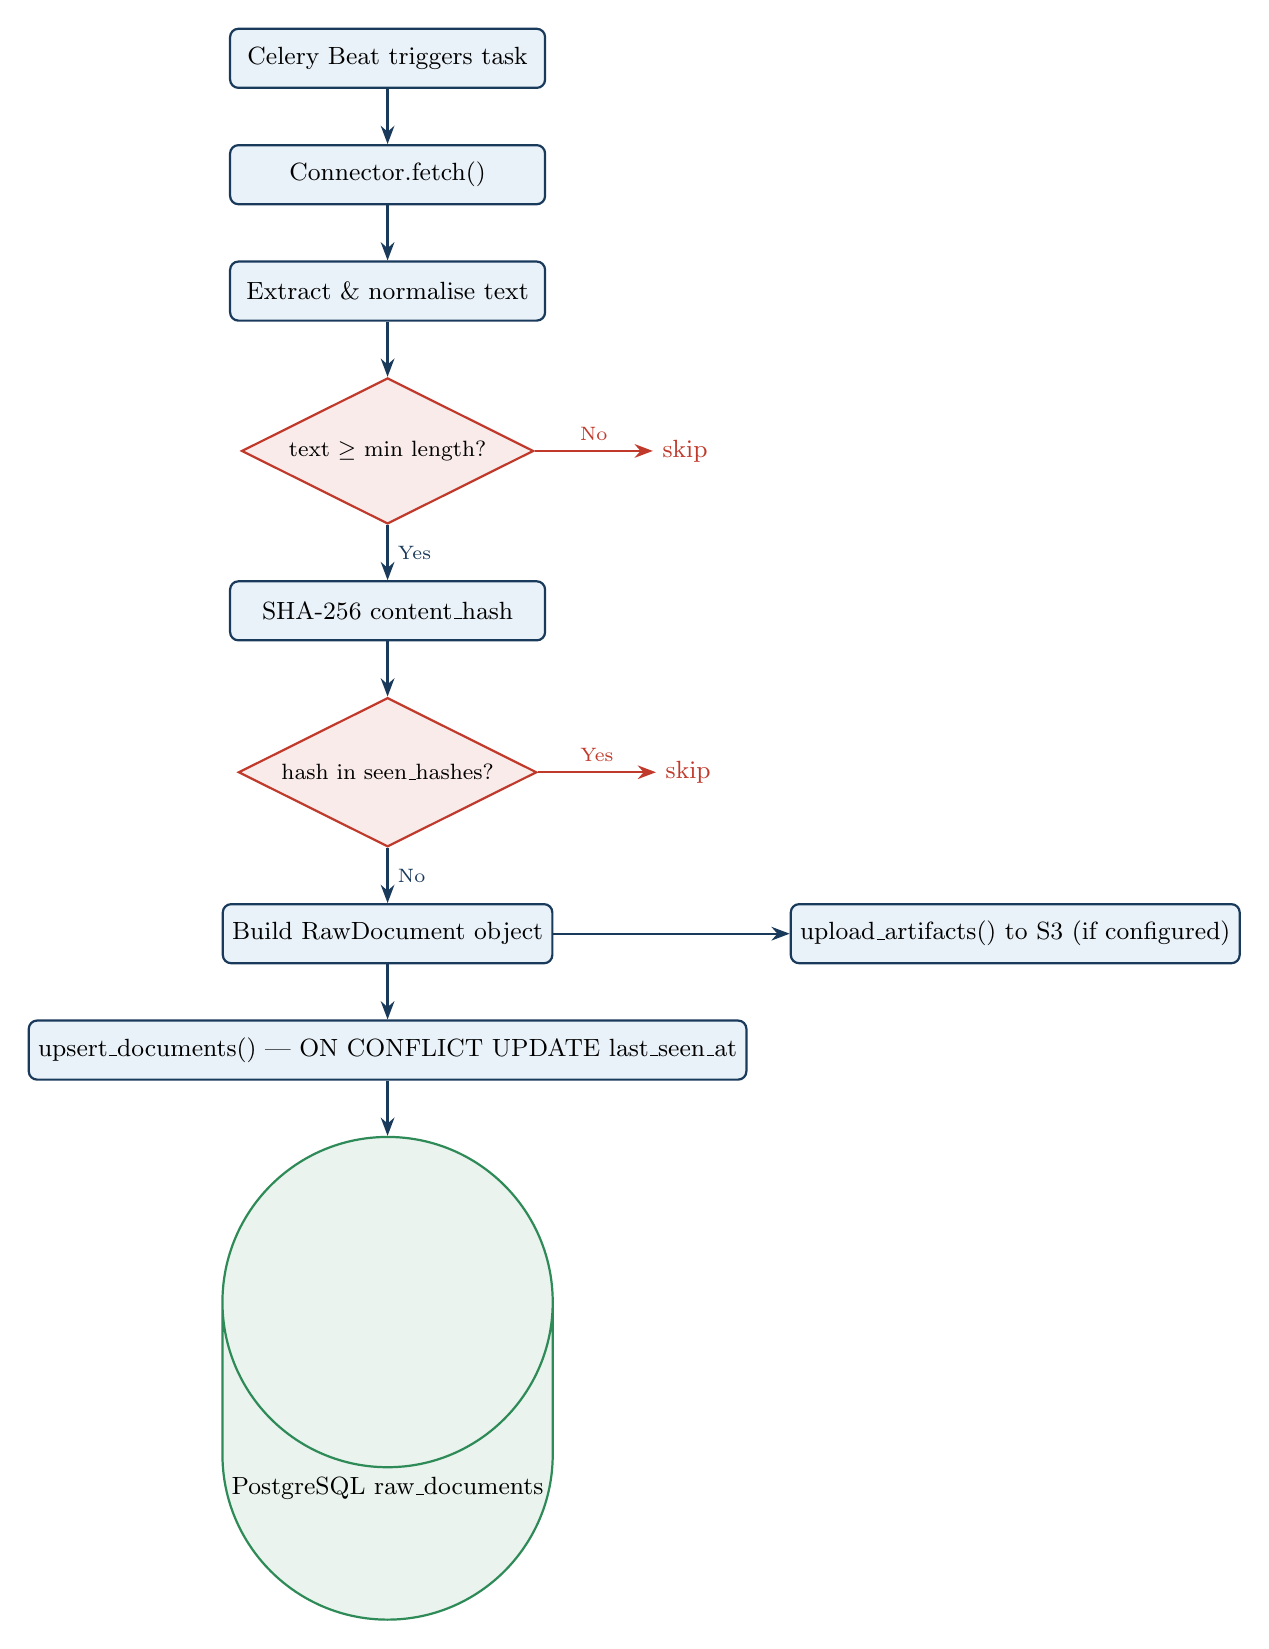
\begin{tikzpicture}[
  node distance=0.7cm,
  every node/.style={font=\small},
  flowstep/.style={
    rectangle, rounded corners=3pt,
    minimum width=4cm, minimum height=0.75cm,
    text centered, draw=primaryblue, thick,
    fill=accentblue!10,
  },
  decision/.style={
    diamond, aspect=2,
    minimum width=3.5cm, minimum height=0.6cm,
    text centered, draw=warnred, thick,
    fill=warnred!10,
    font=\footnotesize,
  },
  store/.style={
    cylinder, shape border rotate=90,
    minimum width=3cm, minimum height=0.8cm,
    text centered, draw=successgreen, thick,
    fill=successgreen!10,
  },
  arrow/.style={-Stealth, thick, color=primaryblue},
]

\node[flowstep]     (trigger)   {Celery Beat triggers task};
\node[flowstep,     below=of trigger]  (connector) {Connector.fetch()};
\node[flowstep,     below=of connector](extract)   {Extract \& normalise text};
\node[decision, below=of extract]  (minlen)    {text $\geq$ min length?};
\node[flowstep,     below=of minlen]   (hash)      {SHA-256 content\_hash};
\node[decision, below=of hash]     (dup)       {hash in seen\_hashes?};
\node[flowstep,     below=of dup]      (doc)       {Build RawDocument object};
\node[flowstep,     below=of doc]      (upsert)    {upsert\_documents() --- ON CONFLICT UPDATE last\_seen\_at};
\node[store,    below=of upsert]   (pg)        {PostgreSQL raw\_documents};
\node[flowstep,     right=3cm of doc]  (s3)        {upload\_artifacts() to S3 (if configured)};

% vertical flow
\draw[arrow] (trigger)   -- (connector);
\draw[arrow] (connector) -- (extract);
\draw[arrow] (extract)   -- (minlen);

% decision: too short -> skip
\node[right=1.5cm of minlen, font=\small, color=warnred] (skip1) {skip};
\draw[arrow, color=warnred] (minlen.east) -- node[above,font=\scriptsize]{No} (skip1);

\draw[arrow] (minlen.south) -- node[right,font=\scriptsize]{Yes} (hash);
\draw[arrow] (hash)   -- (dup);

% decision: duplicate -> skip
\node[right=1.5cm of dup, font=\small, color=warnred] (skip2) {skip};
\draw[arrow, color=warnred] (dup.east) -- node[above,font=\scriptsize]{Yes} (skip2);

\draw[arrow] (dup.south) -- node[right,font=\scriptsize]{No} (doc);
\draw[arrow] (doc)    -- (upsert);
\draw[arrow] (upsert) -- (pg);

% S3 branch
\draw[arrow] (doc.east) -- (s3);

\end{tikzpicture}
\caption{Data flow from source to storage}\label{fig:dataflow}
\end{figure}

\subsection{Step-by-Step Description}

\begin{enumerate}[leftmargin=*, noitemsep]
  \item \textbf{Trigger:} Celery Beat fires a task (e.g.\ \texttt{rss\_ingest\_task}) on its configured schedule.
  \item \textbf{Fetch:} The appropriate connector downloads content from the remote source. Web pages are rendered via Playwright. RSS feeds are parsed by feedparser. PDFs are downloaded via httpx and extracted by pdfplumber or Docling. XML is fetched and parsed by lxml.
  \item \textbf{Extract \& Normalise:} Raw text is extracted. For web pages, Readability-processed markdown is used; if too sparse, the LLM fallback runs. For RSS, title+summary+link are concatenated. For PDFs, text is extracted per page including tables. For XML, section text is gathered recursively with \texttt{itertext()}.
  \item \textbf{Minimum-length filter:} Content shorter than a connector-specific threshold (20--200 characters depending on connector) is discarded.
  \item \textbf{SHA-256 hash:} The normalised \texttt{raw\_text} is hashed with SHA-256.
  \item \textbf{In-run deduplication:} The hash is checked against a \texttt{seen\_hashes} set maintained for the current run. Duplicates within the same fetch cycle are dropped before any database call.
  \item \textbf{RawDocument construction:} A \texttt{RawDocument} SQLModel instance is built with all fields populated.
  \item \textbf{Upsert:} \texttt{upsert\_documents()} executes a PostgreSQL \texttt{INSERT \ldots ON CONFLICT DO UPDATE} statement. New documents are inserted; existing ones (same hash) have only \texttt{last\_seen\_at} updated.
  \item \textbf{S3 upload (optional):} If AWS credentials and a bucket are configured, raw HTML and/or extracted text are uploaded to S3 under the key pattern \texttt{artifacts/\{source\_type\}/\{YYYY-MM-DD\}/\{hash[:8]\}\_raw.html}.
\end{enumerate}

% ═════════════════════════════════════════════════════════════════════════════
\section{URL Normalisation and Spider-Trap Detection (T2.7)}
% ═════════════════════════════════════════════════════════════════════════════

\subsection{Overview}

URL normalisation and spider-trap detection are implemented in \texttt{app/ingestion/url\_utils.py} and are called by the WebConnector before adding any discovered link to the BFS queue.

\subsection{URL Normalisation}

The \texttt{normalize\_url()} function produces a stable, canonical URL form through the following transformation pipeline:

\begin{enumerate}[noitemsep]
  \item \textbf{Relative URL resolution:} If a \texttt{base\_url} is provided, relative URLs are resolved against it using \texttt{urllib.parse.urljoin}.
  \item \textbf{Scheme validation:} Only \texttt{http} and \texttt{https} schemes are accepted; everything else (\texttt{ftp://}, \texttt{mailto:}, \texttt{javascript:}, etc.) returns \texttt{None}.
  \item \textbf{Tracking parameter removal:} 18 known tracking parameters are stripped from the query string.
  \item \textbf{Parameter sorting:} Remaining query parameters are sorted alphabetically for a consistent canonical form (e.g.\ \texttt{?b=2\&a=1} $\to$ \texttt{?a=1\&b=2}).
  \item \textbf{Fragment removal:} The \texttt{\#fragment} component is always removed.
  \item \textbf{Case normalisation:} Scheme and host are lowercased.
  \item \textbf{Trailing slash removal:} Trailing slashes are removed from the path component (except the root \texttt{/}).
\end{enumerate}

The full set of stripped tracking parameters includes:

\begin{lstlisting}[style=pythonstyle, caption={Tracking parameters stripped during normalisation}]
_TRACKING_PARAMS: frozenset[str] = frozenset({
    "utm_source", "utm_medium", "utm_campaign", "utm_term",
    "utm_content", "utm_id", "utm_referrer",
    "fbclid", "gclid", "msclkid", "ttclid",
    "_ga", "_gl", "ref", "referrer", "mc_cid", "mc_eid",
})
\end{lstlisting}

\subsection{Domain Boundary Enforcement}

\texttt{is\_same\_domain(url, allowed\_domain)} returns \texttt{True} only if the URL's host is exactly \texttt{allowed\_domain} or a subdomain of it. Both sides are stripped of a leading \texttt{www.} for stable comparison, preventing false positives.

\begin{lstlisting}[caption={Domain boundary check examples}]
is_same_domain("https://www.cbp.gov/trade/rules", "cbp.gov")  # True
is_same_domain("https://evil.com/cbp.gov", "cbp.gov")          # False
is_same_domain("https://api.fca.org.uk/data", "fca.org.uk")    # True
\end{lstlisting}

\subsection{Spider-Trap Detection}

\texttt{is\_spider\_trap(url)} returns \texttt{True} if any of four trap signatures are detected:

\begin{table}[H]
\centering
\caption{Spider-Trap Detection Rules}\label{tab:trapdetect}
\begin{tabularx}{\textwidth}{@{}l X X@{}}
\toprule
\textbf{Rule} & \textbf{Trigger Condition} & \textbf{Example} \\
\midrule
URL length     & URL longer than 512 characters & Long concatenated parameter strings \\
Session ID     & Query string contains \texttt{session\_id}, \texttt{sid}, \texttt{jsessionid}, \texttt{phpsessid}, \texttt{aspsessionid} & \texttt{/page?sessionid=abc123} \\
Calendar loop  & Path contains a date segment \texttt{/YYYY/MM(/DD)?/} & \texttt{/news/2024/01/15/} \\
Repeated path  & Same path segment repeated 3+ times & \texttt{/a/b/a/b/a/b/} \\
\bottomrule
\end{tabularx}
\end{table}

Calendar-loop detection uses the regex \texttt{/\textbackslash d\{4\}/(?:0[1-9]|1[0-2])(?:/...)?(?:/|\$)} which matches year/month and optional day segments. Repeated-segment detection uses \texttt{(/[\string^/?{\#}]\{2,\})\textbackslash 1\{2,\}} which catches any path segment repeated two or more additional times.

% ═════════════════════════════════════════════════════════════════════════════
\section{Deduplication Mechanism}
\label{sec:dedup}
% ═════════════════════════════════════════════════════════════════════════════

\subsection{Design}

Every \texttt{RawDocument} carries a \textbf{SHA-256 hex digest} of its \texttt{raw\_text} content in the \texttt{content\_hash} column. This 64-character string is the deduplication key at every level of the system.

\begin{lstlisting}[caption={SHA-256 content hash computation (shared across all connectors)}]
def _sha256(text: str) -> str:
    return hashlib.sha256(
        text.encode("utf-8", errors="replace")
    ).hexdigest()
\end{lstlisting}

\subsection{Three-Layer Deduplication}

\begin{enumerate}[noitemsep]
  \item \textbf{Within-run deduplication:} Each connector maintains a \texttt{seen\_hashes: set[str]} in memory during a single \texttt{fetch()} call. Any document whose hash is already in the set is skipped immediately, preventing redundant DB calls.

  \item \textbf{Database-level deduplication:} The \texttt{raw\_documents} table has a \texttt{UNIQUE} constraint on \texttt{content\_hash}. The storage layer uses a PostgreSQL \texttt{INSERT \ldots ON CONFLICT DO UPDATE} (upsert) statement that, on collision, only updates \texttt{last\_seen\_at}. This means a document seen again does not produce a duplicate row but its last-seen timestamp is refreshed.

  \item \textbf{Cross-run identity:} Because the hash is derived from the full text content and not the URL, two different URLs with identical content will correctly deduplicate to a single row. Conversely, the same URL with changed content will produce a new row.
\end{enumerate}

\subsection{Upsert Implementation}

\begin{lstlisting}[caption={PostgreSQL upsert in storage.py}]
stmt = (
    pg_insert(RawDocument)
    .values(
        id=doc.id,
        source_url=doc.source_url,
        source_type=doc.source_type,
        raw_text=doc.raw_text,
        title=doc.title,
        language=doc.language,
        content_hash=doc.content_hash,
        fetched_at=doc.fetched_at,
        last_seen_at=now,
    )
    .on_conflict_do_update(
        constraint="uq_raw_document_content_hash",
        set_={"last_seen_at": now},
    )
)
\end{lstlisting}

\subsection{Robustness Properties}

\begin{itemize}[noitemsep]
  \item \textbf{Idempotent:} Re-running any ingestion task for the same unchanged source produces no new database rows.
  \item \textbf{Race-condition safe:} The PostgreSQL \texttt{ON CONFLICT} clause is atomic; concurrent Celery worker processes cannot produce duplicate rows from simultaneous inserts of the same hash.
  \item \textbf{Content-addressed:} Minor formatting changes that alter the text (e.g.\ a regulatory body updates its website navigation structure) will produce a new hash and a new row. The \texttt{last\_seen\_at} column tracks when a hash was last observed, enabling future change-detection logic.
\end{itemize}

% ═════════════════════════════════════════════════════════════════════════════
\section{S3 Artifact Storage (T2.9)}
% ═════════════════════════════════════════════════════════════════════════════

\subsection{Purpose}

S3 artifact storage preserves the raw HTML and extracted text of fetched documents for audit, replay, and debugging. It is entirely optional; if AWS credentials are not configured, the upload is silently skipped.

\subsection{Key Naming Convention}

\begin{verbatim}
artifacts/{source_type}/{YYYY-MM-DD}/{content_hash[:8]}_raw.html
artifacts/{source_type}/{YYYY-MM-DD}/{content_hash[:8]}_text.txt
\end{verbatim}

The first 8 hex characters of the content hash act as a short identifier. The date prefix organises artifacts chronologically and enables S3 lifecycle policies (e.g.\ transition to Glacier after 90 days).

\subsection{Example S3 URIs}

\begin{lstlisting}[style=shellstyle]
s3://regwatch-artifacts/artifacts/web/2026-03-27/a1b2c3d4_raw.html
s3://regwatch-artifacts/artifacts/rss/2026-03-27/e5f6a7b8_text.txt
s3://regwatch-artifacts/artifacts/pdf/2026-03-27/c9d0e1f2_text.txt
\end{lstlisting}

\subsection{Configuration}

\begin{table}[H]
\centering
\caption{S3 Configuration Environment Variables}\label{tab:s3env}
\begin{tabularx}{\textwidth}{@{}l l X@{}}
\toprule
\textbf{Variable} & \textbf{Default} & \textbf{Description} \\
\midrule
\texttt{AWS\_S3\_BUCKET}          & (empty) & Target S3 bucket name; if empty, uploads are skipped \\
\texttt{AWS\_REGION}              & us-east-1 & AWS region \\
\texttt{AWS\_ACCESS\_KEY\_ID}     & (empty) & AWS access key \\
\texttt{AWS\_SECRET\_ACCESS\_KEY} & (empty) & AWS secret key \\
\bottomrule
\end{tabularx}
\end{table}

If boto3 is not installed or credentials are missing, the \texttt{\_get\_s3\_client()} function returns \texttt{(None, None)} and the upload function returns an empty dict without raising an exception.

% ═════════════════════════════════════════════════════════════════════════════
\section{Monitored Regulatory Sources}
% ═════════════════════════════════════════════════════════════════════════════

\subsection{Configured Sources}

Table~\ref{tab:sources} lists all regulatory sources currently configured in the Celery Beat schedule.

\begin{table}[H]
\centering
\caption{Active Regulatory Sources}\label{tab:sources}
\begin{tabularx}{\textwidth}{@{}l l l l X@{}}
\toprule
\textbf{Authority} & \textbf{Jurisdiction} & \textbf{Connector} & \textbf{Schedule} & \textbf{URL} \\
\midrule
FCA           & UK       & RSS  & 30 min & \texttt{fca.org.uk/news/rss.xml} \\
FCA           & UK       & Web  & 6 h    & \texttt{www.fca.org.uk/news} \\
EUR-Lex       & EU       & Web  & 6 h    & \texttt{eur-lex.europa.eu/latest-laws/} \\
GovInfo       & US       & RSS  & 30 min & \texttt{govinfo.gov/rss/fr.xml} \\
Federal Register & US    & Web  & 6 h    & \texttt{federalregister.gov/documents/current} \\
\bottomrule
\end{tabularx}
\end{table}

\subsection{Financial Conduct Authority (FCA)}

The FCA is the UK's primary financial services regulator. Its news RSS feed (\texttt{fca.org.uk/news/rss.xml}) provides policy statements, guidance consultations, enforcement notices, and market watch updates. The web crawler targets the FCA news index page and discovers linked articles. The FCA source accounts for the majority of the RSS data collected.

\subsection{EUR-Lex}

EUR-Lex is the official portal for European Union law, hosting the Official Journal of the EU, EU regulations, directives, decisions, and legal acts. The web crawler seeds from \texttt{eur-lex.europa.eu/latest-laws/} at a conservative rate of 0.5 RPS (one request every 2 seconds) to respect server capacity. EUR-Lex documents are often available as both HTML and structured PDF, with some in Akoma Ntoso XML format (handled by the XMLConnector).

\subsection{Federal Register / GovInfo (US)}

The Federal Register is the official daily journal of the US federal government, publishing proposed and final rules, executive orders, and notices from all federal agencies. Two collection paths exist: the RSS feed at \texttt{govinfo.gov/rss/fr.xml} provides a daily summary, and the web crawler targets \texttt{federalregister.gov/documents/current} for full document text. GovInfo also publishes USLM-formatted XML (handled by the XMLConnector).

% ═════════════════════════════════════════════════════════════════════════════
\section{Current Data Collection Status}
% ═════════════════════════════════════════════════════════════════════════════

\subsection{Documents Collected}

As of March 2026, the \texttt{raw\_documents} table contains \textbf{188 documents}. Table~\ref{tab:datacounts} provides a breakdown by source type.

\begin{table}[H]
\centering
\caption{Raw Documents by Source Type (March 2026)}\label{tab:datacounts}
\begin{tabular}{@{}l r r@{}}
\toprule
\textbf{Source Type} & \textbf{Count} & \textbf{Percentage} \\
\midrule
RSS   & 122 & 64.9\% \\
Web   & 60  & 31.9\% \\
XML   & 4   & 2.1\%  \\
PDF   & 2   & 1.1\%  \\
Email & 0   & 0.0\%  \\
\midrule
\textbf{Total} & \textbf{188} & \textbf{100\%} \\
\bottomrule
\end{tabular}
\end{table}

\subsection{Analysis}

\begin{itemize}[noitemsep]
  \item \textbf{RSS dominates} because both FCA and GovInfo RSS feeds are polled every 30 minutes and each provides up to 100 entries per cycle. RSS is the highest-velocity source.
  \item \textbf{Web crawler documents} (60) come from the EUR-Lex, FCA, and Federal Register web crawls. At 50 pages per 6-hour run, growth from the web connector is steady but more conservative.
  \item \textbf{XML documents} (4) represent a small number of manually triggered or test runs of the XMLConnector against USLM-formatted Federal Register XML.
  \item \textbf{PDF documents} (2) represent manually triggered PDF test runs.
  \item \textbf{Email documents} (0) is expected: the EmailConnector requires IMAP credentials which are not configured in the current deployment.
\end{itemize}

\begin{successbox}[Ingestion Status]
All automated connectors (RSS, Web) are operational and collecting data continuously. The deduplication mechanism is working correctly: repeated runs do not create duplicate rows. The 188 documents represent 188 \emph{unique} content hashes.
\end{successbox}

% ═════════════════════════════════════════════════════════════════════════════
\section{Application Configuration}
% ═════════════════════════════════════════════════════════════════════════════

All configuration is managed via environment variables, loaded by Pydantic Settings. A \texttt{.env} file can override defaults for local development.

\begin{table}[H]
\centering
\caption{Application Environment Variables}\label{tab:envvars}
\begin{tabularx}{\textwidth}{@{}l l X@{}}
\toprule
\textbf{Variable} & \textbf{Default} & \textbf{Description} \\
\midrule
\texttt{APP\_NAME}                & Regulatory Watch & Application name \\
\texttt{APP\_VERSION}             & 0.1.0            & API version string \\
\texttt{DEBUG}                    & false            & Enable SQLAlchemy query logging \\
\texttt{DATABASE\_URL}            & postgresql://regwatch:\ldots@db:5432/regwatch & PostgreSQL DSN \\
\texttt{REDIS\_URL}               & redis://redis:6379/0 & Redis connection URL \\
\texttt{KAFKA\_BOOTSTRAP\_SERVERS}& kafka:29092      & Kafka broker addresses \\
\texttt{OPENROUTER\_API\_KEY}     & (empty)          & OpenRouter API key for LLM fallback \\
\texttt{OPENROUTER\_MODEL}        & qwen/qwen3-next-80b-\ldots & Model identifier \\
\texttt{OPENROUTER\_BASE\_URL}    & https://openrouter.ai/api/v1 & OpenRouter base URL \\
\texttt{AWS\_S3\_BUCKET}          & (empty)          & S3 bucket for artifacts \\
\texttt{AWS\_REGION}              & us-east-1        & AWS region \\
\texttt{AWS\_ACCESS\_KEY\_ID}     & (empty)          & AWS credentials \\
\texttt{AWS\_SECRET\_ACCESS\_KEY} & (empty)          & AWS credentials \\
\texttt{IMAP\_HOST}               & (empty)          & IMAP server hostname \\
\texttt{IMAP\_PORT}               & 993              & IMAP port \\
\texttt{IMAP\_USER}               & (empty)          & IMAP login user \\
\texttt{IMAP\_PASSWORD}           & (empty)          & IMAP password \\
\texttt{IMAP\_MAILBOX}            & INBOX            & IMAP folder \\
\bottomrule
\end{tabularx}
\end{table}

% ═════════════════════════════════════════════════════════════════════════════
\section{Operational Procedures}
% ═════════════════════════════════════════════════════════════════════════════

\subsection{Starting the Stack}

\begin{lstlisting}[style=shellstyle, caption={Start all services}]
cd regulation-prj-v1
docker compose up --build -d
\end{lstlisting}

\subsection{Running Migrations}

\begin{lstlisting}[style=shellstyle, caption={Apply Alembic migrations}]
docker compose exec api alembic upgrade head
\end{lstlisting}

\subsection{Checking Celery Tasks}

Flower is available at \texttt{http://localhost:5555}. It provides real-time monitoring of:
\begin{itemize}[noitemsep]
  \item Active, scheduled, and completed tasks.
  \item Worker status and concurrency.
  \item Task failure rates and retry counts.
  \item Per-task execution time statistics.
\end{itemize}

\subsection{Triggering Manual Ingestion}

Individual ingestion tasks can be triggered manually from a Python shell or via Celery's API:

\begin{lstlisting}[caption={Trigger a manual RSS poll}]
from app.celery_app import rss_ingest_task
result = rss_ingest_task.delay(
    feed_url="https://www.fca.org.uk/news/rss.xml"
)
print(result.get(timeout=60))
# {'feed_url': '...', 'fetched': 50, 'inserted': 12, 'updated': 38}
\end{lstlisting}

\begin{lstlisting}[caption={Trigger a manual PDF extraction}]
from app.celery_app import pdf_ingest_task
pdf_ingest_task.delay(
    source="https://www.fca.org.uk/publication/policy/ps21-3.pdf",
    title="FCA Policy Statement PS21/3"
)
\end{lstlisting}

\subsection{Heartbeat Monitoring}

A dedicated heartbeat task runs every 5 minutes, pings both Redis and PostgreSQL, and logs a structured JSON status line. The log can be monitored to detect infrastructure-level failures.

% ═════════════════════════════════════════════════════════════════════════════
\section{What is Working and What is Not Yet Implemented}
\label{sec:roadmap}
% ═════════════════════════════════════════════════════════════════════════════

\subsection{Implemented and Functional}

\begin{successbox}[Fully Operational]
\begin{itemize}[noitemsep]
  \item Full Docker Compose stack: PostgreSQL, Redis, Zookeeper, Kafka, FastAPI, Celery Worker + Beat, Flower.
  \item All 5 ingestion connectors: Web (Crawl4AI + Playwright), RSS (feedparser), PDF (pdfplumber + Docling), XML (lxml / USLM / AKN), Email (IMAP).
  \item SHA-256 content deduplication with PostgreSQL upsert (three-layer).
  \item URL normalisation: tracking parameter removal, fragment stripping, parameter sorting, case normalisation.
  \item Spider-trap detection: URL length cap, session ID detection, calendar loop detection, repeated path segment detection.
  \item Domain boundary enforcement in the web crawler.
  \item robots.txt compliance in the web crawler.
  \item Configurable rate limiting (per domain, per connector).
  \item Language detection (ISO 639-1) via langdetect.
  \item S3 artifact storage (boto3, optional).
  \item Alembic database migrations (2 migrations applied).
  \item Structured JSON logging via python-json-logger.
  \item Health-check REST endpoints (\texttt{/health}, \texttt{/health/db}, \texttt{/health/redis}).
  \item Domain CRUD REST API (\texttt{/domains}).
  \item Celery task retry with exponential backoff (up to 3 retries).
  \item 188 real regulatory documents already collected.
  \item LLM fallback (OpenRouter/Qwen) for sparse web pages (requires API key).
\end{itemize}
\end{successbox}

\subsection{Not Yet Implemented}

\begin{warnbox}[Planned Features --- Not Yet Implemented]
\begin{enumerate}[noitemsep]
  \item \textbf{Full-text search:} No search endpoint exists. The \texttt{raw\_documents} table lacks a full-text search index (\texttt{tsvector}/\texttt{GIN}). Planned: \texttt{GET /documents?q=\{query\}} endpoint backed by PostgreSQL FTS or Elasticsearch.
  \item \textbf{AI analysis pipeline:} No LLM summarisation, topic extraction, or regulatory impact analysis has been built. The Kafka bus is provisioned and waiting. Planned: a Kafka consumer reads from the \texttt{raw\_documents} topic, calls an LLM, and writes structured analysis to an \texttt{analysed\_documents} table.
  \item \textbf{Change detection / diff engine:} No mechanism currently identifies when a previously seen document has changed in content. The \texttt{last\_content\_hash} on the \texttt{urls} table supports this, but the diff logic is not implemented.
  \item \textbf{Alerting and notifications:} No email, Slack, or webhook alerts are sent when new regulatory content is detected. Planned: a notification service that watches the Kafka topic and dispatches alerts.
  \item \textbf{User-facing frontend/UI:} No web interface exists. The FastAPI Swagger UI (\texttt{/docs}) is the only browser interface.
  \item \textbf{Document REST API:} No \texttt{/documents} endpoint exists for querying collected documents.
  \item \textbf{Relevance scoring:} The \texttt{relevance\_score} and \texttt{hub\_score} columns on \texttt{urls} are populated with defaults but not yet computed by any algorithm.
  \item \textbf{Email connector scheduling:} The EmailConnector is functional but no Beat periodic schedule is configured.
  \item \textbf{Authentication / authorisation:} The FastAPI application has no auth. All endpoints are publicly accessible. OAuth2/JWT is planned.
  \item \textbf{Metrics and observability:} No Prometheus metrics endpoint. No distributed tracing (OpenTelemetry). Only structured JSON logs are currently available.
  \item \textbf{Multi-replica worker scaling:} The Beat scheduler is embedded in the worker process, which prevents horizontal scaling. Separation of Beat into a standalone service is needed for production.
  \item \textbf{RSS pagination:} The RSS connector is capped at 100 entries per poll. Historical backfill of older feed entries is not implemented.
\end{enumerate}
\end{warnbox}

% ═════════════════════════════════════════════════════════════════════════════
\section{Security Considerations}
% ═════════════════════════════════════════════════════════════════════════════

\begin{itemize}[noitemsep]
  \item \textbf{Credentials:} All secrets (database passwords, AWS keys, IMAP password, OpenRouter API key) are passed as environment variables, not hardcoded. Production deployments should use Docker secrets or a vault solution.
  \item \textbf{robots.txt:} The web crawler respects robots.txt. Non-200 responses are treated as ``allow all'' to handle WAF-blocked robots.txt files, which is a pragmatic compromise. A stricter policy may be appropriate for some jurisdictions.
  \item \textbf{Rate limiting:} Per-domain rate limits are configurable (default: 1 RPS; crawl tasks use 0.5 RPS for regulatory sites). This reduces load on target servers and lessens the risk of IP blocking.
  \item \textbf{User agent:} A transparent user agent string is used: \texttt{RegulatoryWatch/1.0 (compliance monitoring bot; +https://github.com/your-org/regulatory-watch)}.
  \item \textbf{CORS:} The API currently allows all origins (\texttt{allow\_origins=["*"]}). This must be restricted for production deployment.
  \item \textbf{No authentication:} All API endpoints are unauthenticated (see Section~\ref{sec:roadmap}).
\end{itemize}

% ═════════════════════════════════════════════════════════════════════════════
\section{Project File Structure}
% ═════════════════════════════════════════════════════════════════════════════

\begin{lstlisting}[style=shellstyle, caption={Repository layout}]
regulation-prj-v1/
|-- app/
|   |-- celery_app.py         # Celery instance, Beat schedule, all tasks
|   |-- config.py             # Pydantic Settings (env vars)
|   |-- database.py           # SQLAlchemy engine, session factory
|   |-- main.py               # FastAPI app, lifespan, middleware, routers
|   |-- models.py             # SQLModel table definitions (5 models)
|   |-- schemas.py            # Pydantic API schemas
|   |-- ingestion/
|   |   |-- base.py           # IngestorBase abstract class
|   |   |-- artifact_store.py # S3 upload helper
|   |   |-- email_connector.py
|   |   |-- pdf_connector.py
|   |   |-- rss_connector.py
|   |   |-- storage.py        # upsert_documents()
|   |   |-- url_utils.py      # normalize_url, is_spider_trap, etc.
|   |   |-- web_connector.py
|   |   `-- xml_connector.py
|   `-- routers/
|       |-- domains.py        # CRUD for /domains
|       `-- health.py         # /health, /health/db, /health/redis
|-- alembic/
|   |-- versions/
|   |   |-- 001_initial_schema.py
|   |   `-- 002_add_raw_documents.py
|   `-- env.py
|-- docs/
|   `-- regulatory_watch_report.tex   (this document)
|-- alembic.ini
|-- docker-compose.yml
|-- Dockerfile
|-- Makefile
|-- requirements.txt
`-- README.md
\end{lstlisting}

% ═════════════════════════════════════════════════════════════════════════════
\section{Conclusion}
% ═════════════════════════════════════════════════════════════════════════════

The Regulatory Watch platform has a solid, production-grade foundation. The ingestion layer is fully operational with five distinct connector types, robust deduplication, URL canonicalisation, spider-trap protection, and S3 artifact persistence. The distributed task infrastructure (Celery + Redis + Beat) runs reliably and has already accumulated 188 unique regulatory documents from the FCA, EUR-Lex, and the US Federal Register.

The system is designed for extension. Adding a new regulatory source requires only configuring a new Beat schedule entry and providing seed URLs or a feed URL. The connector abstraction ({\tt IngestorBase}) makes it straightforward to add new source types (e.g.\ a GraphQL connector, a scraper for a specific agency's API).

The next major milestones are:
\begin{enumerate}[noitemsep]
  \item Implementing the document retrieval REST API (\texttt{/documents}) with full-text search.
  \item Building the Kafka-based AI analysis pipeline for summarisation and topic tagging.
  \item Implementing change detection and regulatory alerting.
  \item Adding authentication and hardening the API for external exposure.
\end{enumerate}

The codebase follows Python best practices throughout: type annotations, async-first design, structured logging, environment-variable configuration, Alembic-managed migrations, and separation of concerns between the connector, storage, and API layers.

% ═════════════════════════════════════════════════════════════════════════════
\appendix
\section{Celery Beat Schedule Reference}
% ═════════════════════════════════════════════════════════════════════════════

\begin{lstlisting}[caption={Full Celery Beat schedule (app/celery\_app.py)}]
celery.conf.beat_schedule = {
    "heartbeat-every-5minutes": {
        "task": "app.celery_app.heartbeat",
        "schedule": 300.0,          # 5 minutes
    },
    "rss-federal-register-every-30min": {
        "task": "app.celery_app.rss_ingest_task",
        "schedule": 1800.0,         # 30 minutes
        "kwargs": {
            "feed_url": "https://www.govinfo.gov/rss/fr.xml",
        },
    },
    "rss-fca-every-30min": {
        "task": "app.celery_app.rss_ingest_task",
        "schedule": 1800.0,
        "kwargs": {
            "feed_url": "https://www.fca.org.uk/news/rss.xml",
        },
    },
    "web-crawl-eur-lex-every-6h": {
        "task": "app.celery_app.web_crawl_task",
        "schedule": 21600.0,        # 6 hours
        "kwargs": {
            "seed_urls": ["https://eur-lex.europa.eu/latest-laws/"],
            "allowed_domain": "eur-lex.europa.eu",
            "max_pages": 50,
            "rate_limit_rps": 0.5,
        },
    },
    "web-crawl-fca-every-6h": {
        "task": "app.celery_app.web_crawl_task",
        "schedule": 21600.0,
        "kwargs": {
            "seed_urls": ["https://www.fca.org.uk/news"],
            "allowed_domain": "www.fca.org.uk",
            "max_pages": 50,
            "rate_limit_rps": 0.5,
        },
    },
    "web-crawl-federal-register-every-6h": {
        "task": "app.celery_app.web_crawl_task",
        "schedule": 21600.0,
        "kwargs": {
            "seed_urls": [
                "https://www.federalregister.gov/documents/current"
            ],
            "allowed_domain": "www.federalregister.gov",
            "max_pages": 50,
            "rate_limit_rps": 0.5,
        },
    },
}
\end{lstlisting}

% ═════════════════════════════════════════════════════════════════════════════
\section{Glossary}
% ═════════════════════════════════════════════════════════════════════════════

\begin{description}[leftmargin=3.5cm, font=\normalfont\bfseries]
  \item[AKN / Akoma Ntoso] OASIS open standard for legal documents in XML, used widely by EU and UN bodies.
  \item[Beat] Celery's built-in periodic task scheduler, analogous to a \texttt{cron} daemon.
  \item[BFS] Breadth-First Search; the traversal algorithm used by the WebConnector to discover and crawl links.
  \item[Celery] Distributed task queue for Python applications, backed by a message broker (Redis here).
  \item[content\_hash] SHA-256 hexadecimal digest of a document's \texttt{raw\_text}; the deduplication key.
  \item[Crawl4AI] Open-source Python library providing an async web crawler backed by Playwright/Chromium.
  \item[EUR-Lex] Official portal for European Union legal texts.
  \item[FCA] Financial Conduct Authority; UK financial services and markets regulator.
  \item[Flower] Real-time Celery monitoring web UI.
  \item[feedparser] Python library for parsing RSS, Atom, and RDF feeds.
  \item[govinfo.gov] US Government Publishing Office repository for federal government information.
  \item[langdetect] Python port of Google's language-detection library; returns ISO 639-1 codes.
  \item[lxml] High-performance Python XML/HTML processing library using libxml2.
  \item[OpenRouter] LLM gateway aggregating multiple AI model providers under a single API.
  \item[pdfplumber] Python library for extracting text and tables from PDF files using pdfminer.six.
  \item[Playwright] Microsoft's browser automation library; used by Crawl4AI for JS rendering.
  \item[RawDocument] The core SQLModel/database entity representing one unique ingested document.
  \item[spider trap] A URL pattern that generates an infinite number of unique URLs, causing a crawler to loop indefinitely.
  \item[SQLModel] Python library combining SQLAlchemy (ORM) and Pydantic (validation) for type-safe database models.
  \item[upsert] An \texttt{INSERT \ldots ON CONFLICT DO UPDATE} database operation; inserts if new, updates if exists.
  \item[USLM] United States Legislative Markup; XML schema used by US Code and Federal Register documents.
\end{description}

\end{document}
